\documentclass[10pt,oneside]{book}
% \usepackage[a4paper, left=20mm,right=20mm,top=20mm,bottom=20mm]{geometry}
\usepackage[a4paper]{geometry}
% \usepackage[utf-8]{inputenc}
\usepackage{amsmath}
\usepackage{amssymb}
\usepackage{graphicx}
\usepackage{hyperref}
\usepackage{mdframed}
\usepackage{titlesec}
\usepackage{xcolor}

%%%%%%%%%%%%%%%%%%%%%%%%%%%%%%%%%%%%%%%%%%%%%%%%%%%%%%%%%%%%%%%%%%%%%%%% Setups
\graphicspath{{./fig/}}

\hypersetup{%
  linktocpage,
  linktoc=all,
}

\newenvironment{book_quote}[1]
{%
  \mdfsetup{%
    frametitle={\colorbox{white}{\space#1\space}},
    frametitleaboveskip=-\ht\strutbox,
  }
  \begin{mdframed}
}
{
  \end{mdframed}
}

\title{Notes of Concepts and Representations in Vision and Cognition}
\author{Jihang Li}
%%%%%%%%%%%%%%%%%%%%%%%%%%%%%%%%%%%%%%%%%%%%%%%%%%%%%%%%%%%%%%%%%%%%%%%%%%%%%%%

\begin{document}
\maketitle
\tableofcontents

%%%%%%%%%%%%%%%%%%%%%%%%%%%%%%%%%%%%%%%%%%%%%%%%%%%%%%%%%%%%%%%%%%%%%%%% Part 1
\part{Low and Mid Level Vision}%


%%%%%%%%%%%%%%%%%%%%%%%%%%%%%%%%%%%%%%%%%%%%%%%%%%%%%%%%%%%%%%%%%%%%%%%% Part 2
\part{Stochastic Grammars in Vision}%
%==================================================================== Chapter 1
\chapter{Overview of Stochastic Grammar}%
\label{sec:1}
Statistical grammar is a framework with \textbf{probabilistic notion} of
grammaticality.

\section{The Origin of Grammars}%
\label{sec:1.1}
Signals $s$ in real world that tend to occur together more frequently than by
chance can be grouped together to form higher order parts of the signal, and
this process can be repeated to form larger parts. This form a vocabulary of
\textbf{``reusable''} parts.

To measure whether a grouping is a good part:
%
\begin{align}
  \label{eq:1.1}
  \log_2 \left( \frac{p(s\vert_{A \cup B})}{p(s\vert_{A}) \cdot p(s\vert_{B})} \right)
\end{align}
%
where $s\vert_{A}$ and $s\vert_{B}$ are two parts of signal $s: D \rightarrow I$,
with $A \subset D$ and $B \subset D$. Two parts of a signal are bound if the
probability of their co-occurrence is significantly \textbf{greater than} the
probability if their occurrence was independent. Example:
%
\begin{figure}[!htpb]
  \centering
  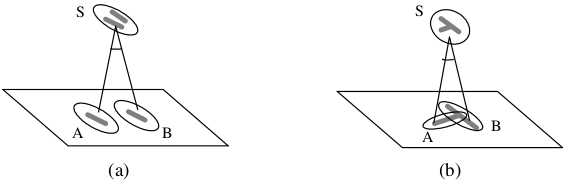
\includegraphics[width=0.7\linewidth]{./fig/fig_1_1.png}
  \caption{(a) Two parallel lines form a reusable part containing as its
    constituents the two lines (b) A T-junction is another reusable part formed
    from two lines.}%
  \label{fig:1.1}
\end{figure}
%

\begin{book_quote}{\textit{Original Texts}}
  The set of such reusable parts is called the \textbf{parse graph} of the
  signal. Firstly, associate to a signal $s$ the set of subsets $\{A_i\}$ of
  $D$ such that $s\vert_{A_i}$ is a reusable part. Then these subsets are made
  into the nodes $\langle A_i \rangle$ of the parse graph. In the graph, the
  proper inclusion of one subset in another, $A_i \subsetneqq A_j$, is shown by
  a ``vertical'' directed edge
  $\langle A_j \rangle \rightarrow \langle A_i \rangle$. For simplicity, we
  prune redundant edges in this graph by adding edges only when
  $A_i \subsetneqq A_j$ and there is no $A_k$ such that
  $A_i \subsetneqq A_k \subsetneqq A_j$.

  \par
  In the ideal situation, parse graph is a tree with the whole signal at the
  top and the domain D (the letters of the text or the pixels of the image) at
  the bottom. Moreover, each node $\langle A_i \rangle$ should be the disjoint
  union of its children, i.e., the parts $\{A_j \vert A_j \subsetneqq A_i\}$
  such that $\cup_j A_j = A_i$.
\end{book_quote}

\section{The Traditional Formulation of Grammar}%
\label{sec:1.2}
Formulation: $\mathcal{G} = (V_N, V_T, \mathbf{R}, S)$, where $V_N$ is a finite
set of non-terminal nodes, $V_T$ is a finite set of terminal nodes, $S \in V_N$
is a start symbol at the root, and \textbf{R} is a set of production rules,
%
\begin{align}
  \label{eq:1.2}
  \mathbf{R} = \{\gamma: \alpha \rightarrow \beta\}
\end{align}
%
where $\alpha, \beta$ are strings that
$\alpha, \beta \in {(V_N \cup V_T)}^+$\footnote{$V^*$ means a string consisting
of $n \geq 0$ symbols from $V$, and $V^+$ means $n \geq 1$} and including at
least one non-terminal symbol.

Chomsky classified languages into 4 types according to the form of their
production rules:

\end{document}
